\begin{abstract}
Public communications described by their publishers as channeling circulate through video platforms, audio archives, transcripts, and written messages. Comparing these records requires distinguishing an upload from a publication, a publisher from a practitioner, and a claimed speaking identity from a verified attribution. We present a working release of Channeling Atlas, a provenance-aware dataset with \SourceCount{} selected publication units, \EditionCount{} retained text-edition records, and \WordCount{} whitespace-delimited words across \ContextCount{} publisher contexts. A separate discovery inventory records \VideoCount{} observed YouTube identifiers and \AccountCount{} account references; it is not a census of channel uploads. The contribution combines typed source lineage, hash-verified acquisition records, explicit missingness, a reproducible descriptive-analysis pipeline, and a dashboard that keeps discovery, acquisition, transcription, and analysis counts separate. We examine lexical topics, context similarity, and sensitivity to document length, identity vocabulary, and collection imbalance. These analyses describe the assembled discourse rather than establish the origin or truth of the communications. The strongest descriptive result is sensitivity to representation: restricting texts to centered 300-word windows substantially changes nearest-neighbor sets. Public metadata and derived results are separated from restricted audio and text. The dataset DOI, human authorship, institutional ethics determination, and annotation validation remain pending; this manuscript is not submission-ready.
\end{abstract}

\section{Introduction}
Video platforms host spiritual instruction, interviews, performances, testimony, and communications attributed to nonhuman or deceased speakers. Publishers may describe these practices as channeling or mediumship. The resulting public record is distributed across platform accounts, independent websites, downloadable audio, edited transcripts, and written editions. A researcher asking how themes vary across publishing communities therefore faces a measurement problem before a modeling problem: the same communication may appear in multiple editions, while a single publishing account may contain several practitioners, claimed identities, or genres.

This problem matters for the study of online religion and cultural communication. Repeated vocabularies can reflect a shared genre, editorial conventions, the same recorded session, interview questions, or a claimed common speaker. A similarity graph that collapses these mechanisms into one edge can invite unsupported conclusions. Likewise, an unavailable video can be mistaken for absent content, and a written message can be mislabeled as speech recognition. These are consequential failures when archives are used to compare small or unfamiliar communities.

Channeling Atlas makes these distinctions explicit. Its present contribution is a documented, purposive research collection and an audit trail for its transformations. The release preserves source links and acquisition outcomes, selects one text edition per documented publication unit for the principal analysis, and records alternative editions without treating them as independent observations. A linked YouTube inventory is retained as discovery metadata rather than forced into a fabricated channel-completion denominator. The paper has three descriptive questions:
\begin{enumerate}
\item Which source types and publisher contexts are represented, and where are acquisition and metadata gaps concentrated?
\item Which lexical patterns appear within and across the selected contexts under a reproducible baseline?
\item How much do those patterns change under length restriction, identity-word masking, and context-balancing controls?
\end{enumerate}
These questions are exploratory. No population-level prevalence estimate, causal mechanism, supernatural-origin test, or clinically meaningful classification is attempted. The dataset's value must be assessed against this bounded scope, rather than a claim to be the first or largest collection of channeling material.

\section{Related Work}
\paragraph{YouTube datasets and sampling.}
YouNiverse documents channel/video collection, language filtering, metadata schema, and sampling bias \citep{ribeiro2021youniverse}. Its sampling-weight analysis depends on external channel ranks; these weights cannot be transferred to a purposive set of publisher pages. The Global YouTube Trending Dataset provides a complementary example of a scheduled, cross-national snapshot design \citep{goncalves2026trending}. Its expected snapshot count permits coverage measurement. Our collection instead has a finite request ledger but lacks a known universe of uploads: completing a declared queue is not equivalent to completing YouTube.

Recent dataset papers also illustrate distinct annotation layers. MetaHarm separates domain-expert, model, and crowdworker labels \citep{jo2025metaharm}; a dataset of Arabic comments on the hijab treats religious discourse through explicitly named annotation dimensions \citep{heraki2025hijab}. These are methodological precedents, not a basis for assigning harm, polarization, or stance labels to the present communities. Our source ledger records publisher-metadata/abstract access for these two papers, separately from the full YouNiverse paper and the Trending dataset author manuscript inspected for structure and collection methods.

\paragraph{Channeling and computational interpretation.}
Recent studies examine semantic correspondence and qualitative structure in prospective communications attributed to extraterrestrial intelligences \citep{wahbeh2026semantic,wahbeh2026qualitative}. Their prospective designs differ from retrospective web-archive construction. Here, identity labels describe what publishers claim; text resemblance does not authenticate those labels. Tube2Vec demonstrates channel-level semantic representations and task-specific validation \citep{boesinger2024tube2vec}, but its large-channel sampling and human evaluation do not transfer to this smaller, heterogeneous archive.

\paragraph{Measurement and documentation.}
Text-as-data research emphasizes alignment between representations and substantive claims \citep{grimmer2013text}. Topic coherence and visually distinct clusters are insufficient evidence of an interpretable taxonomy \citep{doogan2021twaddle,schroeder2025reliability}. Social-data biases arise throughout collection, processing, and interpretation \citep{olteanu2019social}. We therefore pair lexical analysis with provenance and sensitivity diagnostics, and document intended uses and exclusions following Datasheets for Datasets \citep{gebru2021datasheets}. FAIR principles guide identifiers, schemas, provenance, and access descriptions \citep{wilkinson2016fair}; FAIR accessibility can include authorization and does not confer redistribution rights.

\section{Scope, Units, and Collection}
\subsection{Sampling and eligibility}
The corpus grew from an existing Bashar index, the Ra archive, user-supplied YouTube subscriptions, and targeted discovery of relevant publisher sites and claimed speakers. The screenshot screening retained 12 of 28 listed subscriptions and excluded 16, including an explicit user-requested exclusion. These decisions are sampling choices, not validated classifications of every account's content. Later discovery expanded the seed set through public links and first-party pages. Inclusion is based on source descriptions of channeling, mediumship, related interviews, or written communications. Comedic and unrelated accounts are not automatically included merely because they share a subscription list.

The active duration rule has no count cap. A five-minute minimum applies only to material positively associated with Bashar; other included mediums have no minimum duration. Unknown durations remain unresolved metadata probes, not automatic exclusions. This asymmetry is recorded as a design artifact and precludes an unadjusted comparison of clip-duration distributions across all groups.

Collection covers reachable, publicly offered records in declared source contexts. A recent first-party crawl attempted 1,239 page requests in 16 publisher contexts, retrieved 1,215 documents, and retained 24 failed or held outcomes. Its exhausted request queue is a bounded operational result, not whole-site or all-upload completeness. Ordinary access to YouTube in the current environment failed before the origin with a proxy CONNECT rejection. The inventory consequently retains historical identifiers and new first-party links, while the current collection reports zero new direct YouTube media downloads. No caption absence, deletion, or private-video status is inferred from that route failure.

\subsection{Separate observational units}
\begin{table}[t]
\centering\small
\begin{tabular}{p{.27\columnwidth}p{.62\columnwidth}}
\toprule
Unit & Meaning and boundary \\
\midrule
Account reference & A platform/channel reference; may be unresolved or alias another reference. \\
Video identifier & Observed YouTube ID; does not imply successful watch-page or media retrieval. \\
Publisher context & A documented source/edition context, distinct from a verified human practitioner. \\
Publication unit & A source publication selected for analysis after documented edition joins. \\
Text edition & A retained text artifact with origin, hash, selection state, and lineage. \\
Media artifact & An encoded file or derivative; neither a unique session nor a transcript by itself. \\
Claimed identity & A publisher-attributed speaker/entity label; not an authenticated entity. \\
\bottomrule
\end{tabular}
\caption{Units that must not share a denominator. Links between them are typed evidence, not assumed equivalences.}
\label{tab:units}
\end{table}

Table~\ref{tab:units} defines the principal units. For example, a page that links a video and an MP3 provides co-occurrence evidence. It does not establish identical audiovisual content, uploader identity, or transcript alignment. A claimed civilization can recur across practitioners without making those practitioners interchangeable. The schema preserves publisher, creator-context, and claimed-label fields separately, with unresolved mappings retained as such.

\subsection{Acquisition and transformation}
The pipeline records source URL, retrieval outcome, artifact hash, text origin, edition identifier, and publication linkage. Publisher-written messages, publisher-labeled transcripts, platform captions, and local automatic speech recognition (ASR) remain separate categories. Text extraction removes markup while retaining source lineage; it does not certify that written text is a verbatim rendering of audio. Prior ASR outputs are inherited with their model/run provenance where available. This release does not claim a new state-of-the-art speech model evaluation or a measured word-error rate.

The latest publisher-audio cohort contains 192 retained files: three original MP3 files and 189 full-duration Opus derivatives. Retained encoded size is 942,245,703 bytes and decoded duration is 160,392.925 seconds (44.55 hours). Original-source hashes and transformation receipts are retained separately from derivative hashes. A smaller encoded representation reduces storage but is lossy and must not be described as a bit-identical original. The cohort's publisher pages reference 190 distinct YouTube IDs; that number does not turn the 192 audios into 190 verified YouTube downloads.

Collection workers use bounded concurrency, resumable checkpoints, explicit disk floors, and independent failure records. A source-level route failure is not multiplied into thousands of purported per-video attempts. Historical logs retain their own operational settings rather than being rewritten to match a later continuation. The public metadata and private artifact manifest support hash verification and recovery after interrupted work.

\section{Dataset Construction and Quality}
\subsection{Edition selection and lineage}
The principal analytical frame contains \SourceCount{} selected publication units, \WordCount{} words, \ContextCount{} publisher contexts, and \CreatorCount{} creator contexts. Its complete edition lineage contains \EditionCount{} rows. The selected-input update combined 493 previously selected editions with 192 new publisher editions. Two new editions matched existing publications by the same individual article URL and whitespace-folded text; the existing selected edition was retained in both cases. Thus 685 selected-input candidates yield 683 publication units. The complete 694-row lineage also preserves nine previously catalogued alternatives, giving 11 non-selected editions overall.

This is conservative edition reconciliation rather than a solution to all near-duplicate detection. Exact encoded-file hashes, normalized text hashes, and publication identifiers answer different questions. Similar topics, similar titles, and a shared claimed speaker are not merge rules. Reposted, translated, edited, or partially overlapping sessions may remain distinct when evidence does not justify a stronger join. Future deduplication must preserve prior source IDs and expose the merge rationale.

\begin{table}[t]
\centering\small
\begin{tabular}{lr}
\toprule
Selected text origin & Units \\
\midrule
Imported machine ASR & 12 \\
Local ASR & 221 \\
Platform automatic caption & 14 \\
Publisher-written message & 226 \\
Retained local ASR & 19 \\
Publisher-labeled transcript PDF & 15 \\
Publisher transcript & 106 \\
Linked publisher caption & 70 \\
\midrule
Total & 683 \\
\bottomrule
\end{tabular}
\caption{Selected-edition provenance. Categories preserve source lineage; neither publisher labeling nor ASR implies human-verified verbatim transcription.}
\label{tab:origins}
\end{table}


\subsection{Missingness and validity}
Text origins are shown in Table~\ref{tab:origins}. The provenance mix is substantively important: an edited transcript may remove disfluencies, a written edition may be composed independently, and ASR may miss unfamiliar names or speech in noise. The corpus has no human reference transcription study. ASR quality, speaker diarization, entity attribution accuracy, and question/answer extraction precision are therefore unmeasured.

Dates are missing for 300 of 683 selected units (43.9\%). Known source dates may refer to publication, upload, recording, or archive edition; they must not be silently treated as the same event time. The YouTube layer contains \VideoCount{} observed IDs and \AccountCount{} account references, but the total uploaded-video denominator is unknown. Historical uploader joins are retained with their own evidence dates; an ID found on a publisher page does not refresh those joins.

Validation checks unique stable identifiers, selected-versus-alternative edition counts, source/body hash consistency, known merge evidence, media-hash semantics, and public-export exclusion of raw source bodies and local paths. These are integrity checks, not content-validity or source-authentication tests. The frame hash and build receipts bind reported counts to a concrete snapshot. Full reconstruction from source speech requires authorized access to retained material; rebuilding public tables from frozen metadata is a narrower reproducibility claim.

\section{Descriptive Analysis and Sensitivity}
\subsection{Representations and design}
Each selected text contributes once to the main fit. The reproducible baseline uses Unicode alphabetic tokens, retained apostrophes, case folding, unigrams/bigrams, sublinear term frequency, minimum document frequency two, and at most 24,000 TF--IDF features. Declared identity phrases are masked for the main analysis. It fits an eight-component non-negative matrix factorization (NMF), and computes clustering diagnostics on a reduced lexical representation. The component count is a declared exploratory setting, not an estimated number of spiritual traditions or true latent entities. Terms and example links describe component vocabulary; any interpretive label remains provisional. Model settings, software versions, random seeds, convergence outcomes, and measured resource use are included in the analysis receipt. The CPU-only managed Linux environment exposes five logical CPUs with a four-CPU-equivalent quota and 32 GiB memory quota (AMD EPYC 9V74); no GPU device was detected. This describes the current analysis environment, not all inherited ASR acquisition runs.

Context comparisons use source-level observations rather than counting every text edition. Pairwise similarity is descriptive and shares documents across pairs, so pair counts are not independent sample sizes. Mutual-neighbor edges represent a stated similarity rule, not social interaction, influence, common authorship, or agreement. The map projection is a display of a high-dimensional representation; distances and apparent islands should be checked against numerical scores.

Three controls test obvious alternative explanations. A centered 300-word view restricts the amount of text per source; an identity-masking contrast removes a declared phrase registry that could mechanically connect records. A balanced-IDF control fits vocabulary and inverse document frequencies on at most ten source units per context, then transforms all 683 units; a separate balanced NMF fit uses the same 107-unit subset. Selection uses source-ID hashes rather than result-driven sampling. Seed comparisons assess numerical stability. Neighbor-set comparisons use top-five sets and Jaccard intersection over union, with both equal-source and equal-context averages. These controls reveal sensitivity within the assembled corpus, not a causal decomposition of genre, practitioner, editing, and belief. Sentence embeddings, where run, are a complementary representation \citep{reimers2019sentencebert}; their agreement with lexical rankings is not a semantic ground-truth score.

\subsection{Snapshot findings}
The two largest publisher contexts contain 203 and 198 selected units, respectively, and together account for 58.7\% of the frame. Eighteen of 26 contexts have fewer than five units, including 11 singleton contexts. Figure~\ref{fig:profile} shows this imbalance alongside text-length differences. The resulting archive is useful for inspecting these records but cannot supply an equal-evidence comparison of every practitioner or claimed civilization.

\begin{figure*}[!t]
\centering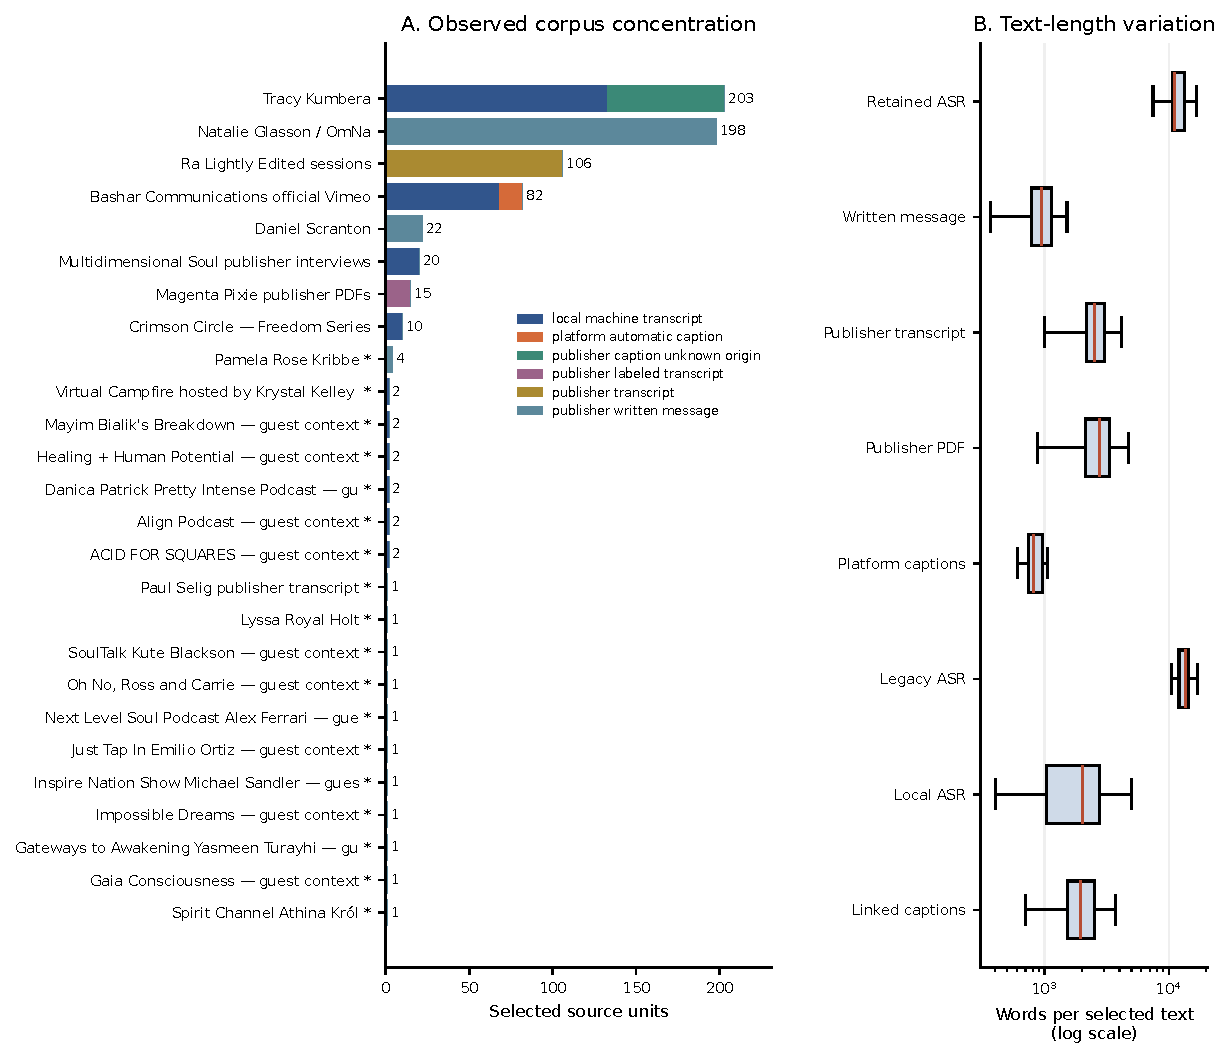
\includegraphics[width=.97\textwidth]{generated/corpus-profile.pdf}
\caption{Selected publication units by publisher context and text-length distributions. Stars mark contexts with fewer than five units. Text-origin colors are provenance categories, not quality rankings. Boxes indicate medians and interquartile ranges; whiskers extend to 1.5 interquartile ranges and outliers are not displayed. These are observed collection counts, not lifetime upload totals.}
\label{fig:profile}
\end{figure*}

The clearest diagnostic is sensitivity to the amount of text represented. Relative to masked full-text TF--IDF, the centered 300-word view has mean top-five neighbor-set Jaccard 0.137 across sources and 0.062 when contexts receive equal weight. Pairwise cosine-rank Spearman correlation is 0.536. Identity masking alone produces source-mean Jaccard 0.787; balanced-IDF fitting produces 0.782. Thus high global rank correlation under some preprocessing changes does not guarantee identical local neighbors, and the much larger length-window change cautions against treating a single similarity map as an intrinsic ordering of communications.

\begin{table}[t]
\centering\small
\begin{tabular}{lrrr}
\toprule
Contrast & $J_s$ & $J_c$ & $\rho$ \\
\midrule
Identity masking & .787 & .940 & .997 \\
Centered 300 words & .137 & .062 & .536 \\
Balanced IDF & .782 & .853 & .991 \\
Lexical vs. MiniLM (300 words) & .118 & .098 & .430 \\
\bottomrule
\end{tabular}
\caption{Top-five neighbor Jaccard averaged equally across sources ($J_s$) or publisher contexts ($J_c$), and rank correlation of pairwise similarities ($\rho$). All comparisons use the same 683-source universe. Pair scores are dependent; these values are not significance tests. The embedding comparison uses matched bounded spans, not full transcripts.}
\label{tab:sensitivity}
\end{table}

The pretrained MiniLM comparison uses the same identity-masked, centered maximum-300-word spans. Complete chunks of at most 240 content wordpieces are encoded without wordpiece truncation and pooled by content length. Its neighbor sets differ substantially from the bounded lexical representation (Table~\ref{tab:sensitivity}); this measures representation disagreement rather than an accuracy advantage. The model revision, encoder hash, and exact-input cache binding are retained. No weights were updated and no model was distilled or fine-tuned.

\begin{figure*}[!t]
\centering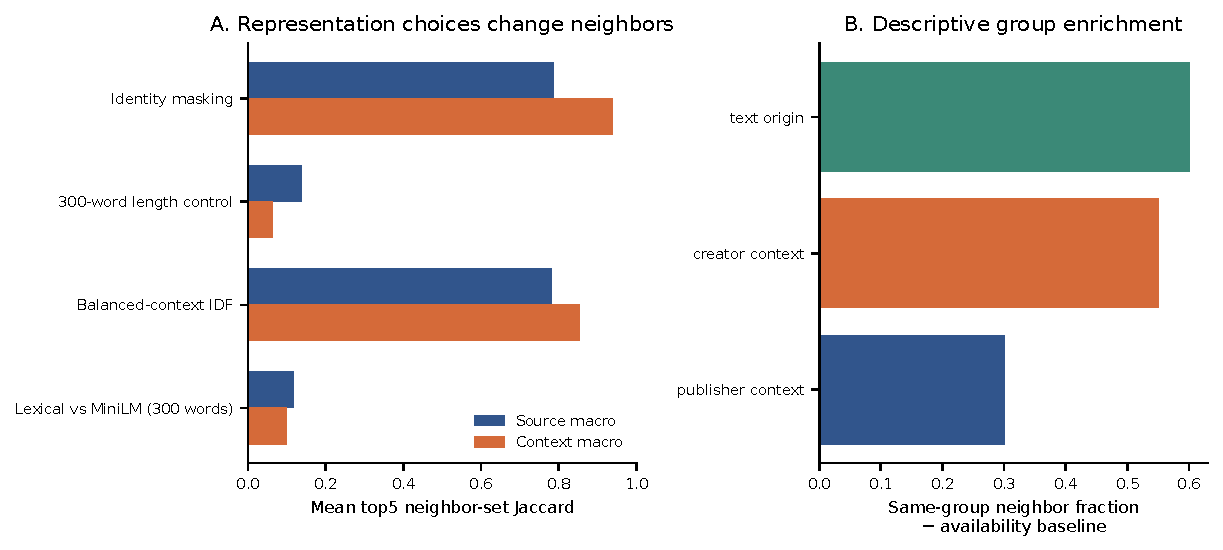
\includegraphics[width=.97\textwidth]{generated/sensitivity.pdf}
\caption{Representation sensitivity and descriptive same-group neighbor enrichment. All top-five comparisons use a common source universe. Enrichment subtracts each group's availability baseline before averaging within and equally across groups. Publisher context, creator context, text origin, and source length are confounded; these are diagnostics, not causal effect estimates.}
\label{fig:sensitivity}
\end{figure*}

NMF results are also conditional on the fit design. The eight-component main fit uses random seed 11; seeds 23 and 47 yield mean matched-component cosines 0.770 and 0.795. The mean hides heterogeneous stability: two seed-47 component matches are only 0.188 and 0.343. Their dominant-component adjusted Rand indices relative to the main fit are 0.666 and 0.737. All three runs converged under a 2,000-iteration limit, with seed 47 requiring 1,126 iterations. A separate balanced fit on 107 units has mean matched-component cosine 0.576, illustrating corpus-composition sensitivity. Figure~\ref{fig:topics} retains top-term labels, including single-letter and discourse fragments such as ``d,'' ``you're,'' and ``yeah.'' These are warnings about vocabulary and format effects, not polished evidence of doctrinal categories.

\begin{figure*}[!t]
\centering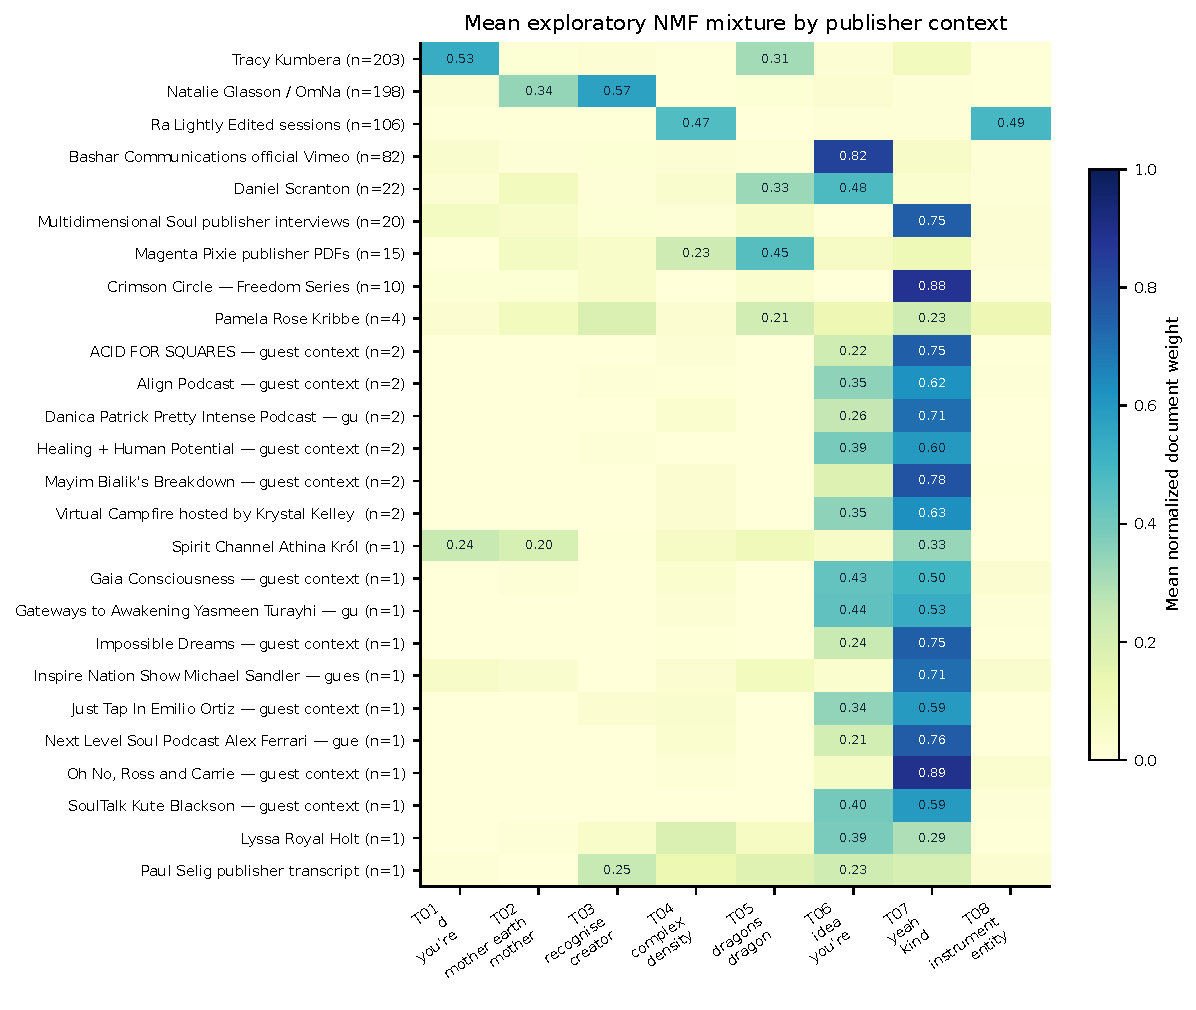
\includegraphics[width=.97\textwidth]{generated/topic-contexts.pdf}
\caption{Mean exploratory eight-component NMF mixtures by publisher context, using masked full-text TF--IDF and seed 11. Each selected source receives equal weight within its context. Labels concatenate top terms, including uninterpretable/discourse artifacts. Low-count rows and seed/composition sensitivity prevent treating these factors as a validated taxonomy.}
\label{fig:topics}
\end{figure*}

The illustrative $k=8$ clustering in normalized 50-dimensional TF--IDF SVD space has cosine silhouette 0.254 at seed 11. Its association with publisher contexts (adjusted Rand index 0.808) and text origins (0.516) underscores possible collection/format effects. Alternative values $k\in\{4,6,10\}$ and three seeds are diagnostic runs, not an optimization yielding a true number of groups. The mutual-five-neighbor graph has 888 undirected edges; these encode lexical proximity only. The two-dimensional view is lossy, and full-space cosine values remain authoritative. The exported context-similarity figure excludes self-pairs and displays contexts with at least five selected units; all 676 context cells and pair denominators remain available in exported tables. That figure, the network, and the projection diagnostics accompany the full public analysis and source ZIP.


The final analysis pass took 51.27 seconds with peak process resident memory 476,728 KiB, reusing an exact-input embedding cache. The separate original embedding pass took 63.64 seconds for 1,366 complete chunks and 245,517 content wordpieces; these are not presented as one cold-start benchmark. The code emits 9,024 punctuation-based question cues, which are explicitly unvalidated and not 9,024 observed question/answer pairs. Inspection of source passages and human transcription/annotation checks remains necessary before semantic interpretation or benchmark use.


\subsection{Questions, answers, and a typed knowledge graph}
The research interface distinguishes printed question/answer turns from question-like cues and generated reading prompts. A question mark or a model-produced query is not sufficient evidence of an interviewer question. A generated summary must retain source identifiers and uncertainty about speaker and boundaries. Answer comparison first retrieves candidate passages, then asks whether the question, speaker attribution, scope, and modality actually match. Lexical similarity alone cannot classify two answers as common, conflicting, or contradictory.

The present release therefore treats a question bank and cross-entity graph as typed research aids, not validated benchmark labels. Historical question-bank outputs retain their own frozen frame and are not advertised as newly validated over all \SourceCount{} units. Meaningful expansion requires a stratified, human-checked sample: printed Q\&A, interview speech, monologue, written messages, short sources, and long sources. Precision of question detection, boundary agreement, answer-supportedness, and inter-annotator agreement should be reported separately. This human evaluation is TBD rather than replaced by a model-panel vote.

\section{Release, Documentation, and Reuse}
\subsection{Artifacts and access levels}
The public package contains document and edition metadata, media receipts, observed YouTube IDs, account references and attribution links, per-context tables, analysis outputs, code, schemas, and this manuscript. A versioned metadata ZIP supplies JSONL/CSV tables, schema, datasheet, rights statement, checksum list, and a DOI-deposit draft; it contains neither full source bodies nor media. JSON/JSONL and CSV expose stable IDs and explicit nulls. The dashboard adds source filters, coverage states, context pages, and links to downloadable numerical outputs. The locally retained source archive contains audio, extracted text, transformation receipts, and collection evidence under restricted access. At this manuscript snapshot, remote private-archive upload has not been verified; no remote archival completion or reviewer-access guarantee is implied. This manuscript does not represent that private archive as an openly redistributable media corpus.

\noindent Public research repository: \url{https://github.com/occult-kranti/channels-ET}.\\
Dataset dashboard: \url{https://occult-kranti.github.io/channels-ET/dist/dataset-submission/}.\\
Dataset DOI: \textbf{TBD; required before ICWSM submission}.\\
Responsible contact and access process: \textbf{TBD with human authorship}.

The public release must be versioned separately from a changing collection workspace. Dataset metadata, hashes, schema, source ledger, and change log support identification and audit. A future DOI deposit should point to an immutable contributed dataset with a clear license and retained metadata even if underlying assets are withdrawn. Reuse terms are asset-specific: the project's own code and derived tables cannot grant a blanket license over third-party audio, text, likenesses, or publisher branding. A public URL is evidence of discoverability, not proof of consent to redistribution.

\subsection{Reproducibility levels}
Three operations are distinguished. First, public-metadata reconstruction regenerates counts and coverage views from the exported snapshot. Second, frozen-analysis inspection reproduces plots and rankings from retained numerical outputs. Third, full text-model recomputation needs the authorized source bodies and pinned analysis environment. Reacquiring the same URL at a later time is a separate operation because platform availability, editions, and captions can change. Each claim should state which level has actually been tested.

\subsection{Research applications}
The collection supports studies of archive selection, text-edition effects, publisher vocabulary, and the organization of public spiritual discourse. An edition-matched analysis can compare written and spoken versions without treating them as independent participants. A study of recurring claimed identities can compare multiple publisher contexts after documenting the attribution evidence and controlling for source format. A retrieval task can ask whether a returned answer is supported by the referenced passage rather than whether it endorses a belief. None of these applications requires treating a claimed nonhuman speaker as established fact.

Useful future experiments include a human-validated ASR error sample across noise and vocabulary conditions; edition-aware retrieval with held-out publications; blinded topic-intrusion or interpretation tasks; and a contradiction benchmark that distinguishes incompatible propositions from differences in scope, uncertainty, or metaphor. These are proposed experiments, not completed findings. Future corpus expansion should reserve evaluation data before iterative prompt or model optimization.

\section{Limitations and Ethical Considerations}
\paragraph{Selection and dependence.}
This is a purposive, access-conditioned collection with substantial context imbalance. It neither represents all practitioners nor establishes total uploads for any channel. Repeated speakers, hosts, editorial staff, source archives, and shared sessions induce dependencies. Fine-grained context labels do not create independent populations. English-oriented tooling and heterogeneous date information further limit linguistic and temporal conclusions.

\paragraph{Attribution and interpretation.}
Source identities are claims in public material. An entity name in a footer, marketing notice, or related-link block can disagree with the communication itself. Labels should be traced to their evidential span and corrected without deleting prior provenance. Topic mixtures and clusters can reflect boilerplate, length, source type, or model behavior. They do not establish extraterrestrial contact, deceased-person identity, predictions, causal influence, dishonesty, or mental health status.

\paragraph{Privacy, rights, and audience expectations.}
Material may include identifiable speakers, audience questions, personal experiences, and sensitive health, spiritual, or biographical information. Availability on a public page does not remove these concerns. Public outputs minimize reproduced source passages and avoid participant profiling; full audio/text remains a separate restricted artifact layer. Human authors must determine consent, institutional review obligations, redistribution rights, takedown procedures, and access criteria. No participant recruitment, compensation, IRB approval, or comprehensive copyright clearance is asserted by this draft.

\paragraph{Automated assistance and review.}
Model agents assisted development and adversarial checking, but their agreement is not human annotation or external peer review. Plausible generated summaries, citations, or graph edges require evidence checks. Source-grounded prose and numerical build receipts reduce some errors but cannot replace subject expertise, listening validation, or review by the represented communities. Human approval of the paper, checklist, release license, and responsible contact remains required before actual submission.

\section{Conclusion}
Channeling Atlas provides a bounded, versioned dataset and analysis workflow for public spiritual media. Its primary contribution is the explicit connection between discovery evidence, publication units, text editions, media artifacts, and analytical uncertainty. The working release enables inspection of lexical structure while making incomplete platform coverage, heterogeneous transcription origins, and access restrictions visible. A submission-ready dataset still requires a persistent deposit, human authorship and ethical determination, and validation proportional to the eventual claims.

\section*{Acknowledgements and Generative AI Disclosure}
ChatGPT/Codex was used to assist source discovery and inspection, draft and revise prose, write code, generate tables and plots from retained data, and coordinate model-agent reviews. Bibliographic metadata and decisive venue passages were checked against retained sources; model agents were not human reviewers. Human author names, institutional affiliations, funding, competing interests, and final approval are TBD. No generative AI system is listed as an author. The disclosure must be updated by the eventual human authors to match the final contribution record.
